\chapter{漂浮与下沉}\label{ch:g1:floating-and-sinking}

把一颗小石子丢进水洼，它会沉到底。把一片树叶丢进去，
它会像一只小船一样浮在水面上。洗澡、玩水洼和池塘，
都在问同一个问题——什么会\omterm{def:g1:floating-and-sinking:words}{漂浮}，什么会\omterm{def:g1:floating-and-sinking:words}{下沉}，
我们能不能在放进水里之前先猜一猜？

\section{漂浮还是下沉？}

\begin{definition}[漂浮与下沉]\label{def:g1:floating-and-sinking:words}
若水能把某物托在水面上，则称该物体\emph{漂浮}\index{漂浮}，
若物体沉到水底，则称它\emph{下沉}\index{下沉}。
木塞会漂浮，小石子会下沉。
\end{definition}

\begin{method}[公平的漂浮测试]\label{met:g1:floating-and-sinking:test}
\begin{enumerate}
  \item 在大碗（或水槽）里装满水；
  \item 轻轻地把物体放到水面上，\emph{轻轻}——不要扔：
        水花可能会把\omterm{def:g1:floating-and-sinking:words}{漂浮}的物体短暂地压进水里；
  \item 完全松手，等待并数到 $5$；
  \item 看一看：浮在上面的是\omterm{def:g1:floating-and-sinking:words}{漂浮}物，沉在底部的是\omterm{def:g1:floating-and-sinking:words}{下沉}物。
\end{enumerate}
每个物体都用同样的方法测试，这样比较才公平。
\end{method}

\begin{example}[试一试：分类游戏]\label{ex:g1:floating-and-sinking:sorting}
找来一个木塞、一枚硬币、一把塑料勺、一把金属勺、一颗小石子、一支
铅笔和一片干树叶，然后用
\cref{met:g1:floating-and-sinking:test}逐个测试。\omterm{def:g1:floating-and-sinking:words}{漂浮}物有：木塞、
塑料勺、铅笔、树叶。\omterm{def:g1:floating-and-sinking:words}{下沉}物有：硬币、金属勺、
小石子。每次放入之前，大声说出你的猜测——
这在科学上叫作\emph{预测}，
猜错也是乐趣的一半。
\end{example}

\begin{omfigure}
\begin{tikzpicture}[scale=0.85]
  \draw[thick] (0,0) -- (0,3.2) (0,0) -- (9,0) (9,0) -- (9,3.2);
  \fill[omDef, opacity=0.15] (0,0) rectangle (9,2.6);
  % cork: a little cylinder riding half-sunk
  \draw[thick, fill=brown!45] (1.25,2.38) rectangle (1.75,2.78);
  \draw[thick, fill=brown!30] (1.5,2.78) ellipse (0.25 and 0.08);
  \node[above, font=\small] at (1.5,3.0) {木塞};
  % leaf: pointed oval with a midrib, flat on the surface
  \draw[thick, green!45!black, fill=green!40]
    (3.6,2.62) .. controls (4.0,2.92) and (4.5,2.92) .. (4.85,2.62)
    .. controls (4.5,2.52) and (4.0,2.52) .. (3.6,2.62);
  \draw[green!45!black] (3.68,2.63) -- (4.78,2.63);
  \draw[thick, green!45!black] (3.6,2.62) -- (3.42,2.56);
  \node[above, font=\small] at (4.2,3.0) {树叶};
  % pencil: yellow body, sharpened tip, lying on the water
  \draw[thick, fill=red!45] (5.95,2.56) rectangle (6.1,2.76);
  \draw[thick, fill=yellow!75] (6.1,2.56) rectangle (7.6,2.76);
  \draw[thick, fill=brown!35] (7.6,2.56) -- (7.95,2.66)
    -- (7.6,2.76) -- cycle;
  \fill[black] (7.95,2.66) -- (7.85,2.62) -- (7.85,2.7) -- cycle;
  \node[above, font=\small] at (6.9,3.0) {铅笔};
  % pebble: an irregular gray lump on the bottom
  \draw[thick, fill=omExo!55]
    (2.25,0.18) .. controls (2.3,0.45) and (2.75,0.52) .. (2.95,0.32)
    .. controls (3.05,0.18) and (2.9,0.04) .. (2.6,0.04)
    .. controls (2.4,0.04) and (2.25,0.06) .. (2.25,0.18);
  \node[above, font=\small] at (2.6,0.6) {小石子};
  % coin: a flat golden disc
  \draw[thick, fill=yellow!70!orange] (5.15,0.04) rectangle (5.65,0.12);
  \draw[thick, fill=yellow!85!orange] (5.4,0.12) ellipse (0.25 and 0.07);
  \node[above, font=\small] at (5.4,0.45) {硬币};
  % metal spoon: bowl plus handle
  \draw[thick, fill=omExo!40] (7.05,0.2) ellipse (0.34 and 0.16);
  \draw[line width=2.4pt, omExo!80!black] (7.38,0.16) -- (8.5,0.08);
  \node[above, font=\small] at (7.8,0.55) {金属勺};
  % the water in front of everything, and its surface line
  \fill[omDef, opacity=0.12] (0,0) rectangle (9,2.6);
  \draw[omDef, thick] (0,2.6) -- (9,2.6);
\end{tikzpicture}

{\small 分类游戏之后：\omterm{def:g1:floating-and-sinking:words}{漂浮}物浮在水面上，
\omterm{def:g1:floating-and-sinking:words}{下沉}物停在水底。}
\end{omfigure}

\begin{omfigure}
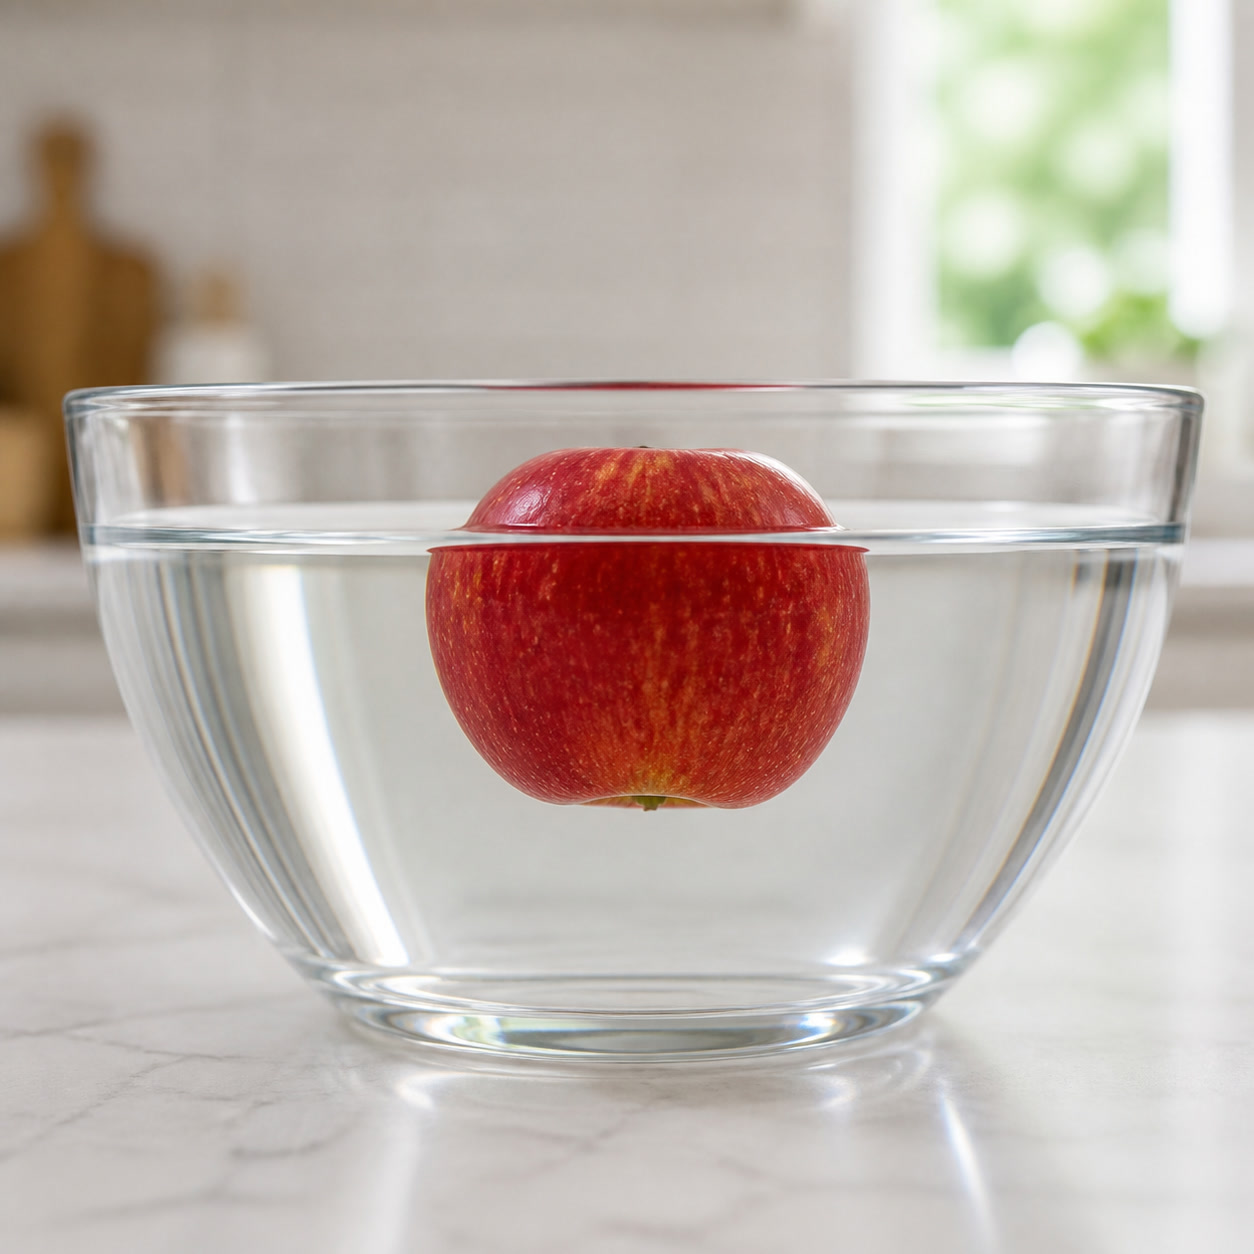
\includegraphics[width=0.42\linewidth]{images/book1/ai/g1-floating-apple.jpg}

{\small 一个苹果\omterm{def:g1:floating-and-sinking:words}{漂浮}在一碗水里：它浮得很低，大部分身体都在水面以下，但它仍然\omterm{def:g1:floating-and-sinking:words}{漂浮}着。}
\end{omfigure}

\section{不只是轻重的问题}

很多人猜测：“重的东西会\omterm{def:g1:floating-and-sinking:words}{下沉}，轻的东西会\omterm{def:g1:floating-and-sinking:words}{漂浮}”。
但水却让他们大吃一惊。

\begin{example}[原木与硬币]\label{ex:g1:floating-and-sinking:log}
一根倒下的树干重得你根本抬不动——可它
却能顺河漂流。一枚小硬币的重量比一块饼干还轻——
可它马上就会沉下去。所以，轻重不能决定一切，
巨大的原木\omterm{def:g1:floating-and-sinking:words}{漂浮}，而小小的硬币却沉没。
\end{example}

\begin{example}[起作用的是材料]\label{ex:g1:floating-and-sinking:stuff}
回想一下分类游戏：塑料勺\omterm{def:g1:floating-and-sinking:words}{漂浮}了，而
金属勺沉下去了，尽管它们形状相同、用途也相同。
造成差别的，是它们所用的\emph{材料}——
木头、木塞和大多数塑料都是\omterm{def:g1:floating-and-sinking:words}{漂浮}材料；金属、石头和
玻璃都是\omterm{def:g1:floating-and-sinking:words}{下沉}材料。物体通常会表现出它所用材料的特性：
无论是小树枝还是整根树干，木头都会\omterm{def:g1:floating-and-sinking:words}{漂浮}。
\end{example}

\begin{remark}[一点小小的疑问]\label{rem:g1:floating-and-sinking:why}
\emph{为什么}木头会\omterm{def:g1:floating-and-sinking:words}{漂浮}，金属会\omterm{def:g1:floating-and-sinking:words}{下沉}？这是一个真正的问题，
它的完整答案是本课程的一个宝藏——它
需要以后几年才会学到的想法。现在我们先收集好的
观察结果；到那时，“为什么”就会等着我们做好准备。
\end{remark}

\section{水会把物体推回来}

\begin{example}[试一试：把球压到水下]\label{ex:g1:floating-and-sinking:push}
在浴缸里拿一个\omterm{def:g1:floating-and-sinking:words}{漂浮}的球，用手掌把它慢慢压入水下。
感觉到了吗？你压得越深，水向上推它的力就越大——
如果手一滑，球就会从水里弹出来。
水并不只是\emph{让}\omterm{def:g1:floating-and-sinking:words}{漂浮}物留在水面上，而是在主动托着它们，
就像你的双手托着一个婴儿。
\end{example}

\begin{omfigure}
\begin{tikzpicture}[scale=0.85]
  \draw[thick] (0,0) -- (0,3.4) (0,0) -- (6.5,0) (6.5,0) -- (6.5,3.4);
  \draw[omDef, thick] (0,2.7) -- (6.5,2.7);
  \fill[omDef, opacity=0.15] (0,0) rectangle (6.5,2.7);
  \draw[thick, fill=white] (3.2,1.5) circle (0.6);
  \node[font=\small] at (3.2,1.5) {球};
  \draw[-Stealth, very thick, omThm] (3.2,3.3) -- (3.2,2.25);
  \node[right, font=\small, omThm] at (3.35,2.9) {手向下压};
  \draw[-Stealth, very thick, omDef] (3.2,0.35) -- (3.2,0.85);
  \node[right, font=\small, omDef] at (3.35,0.55) {水向上推};
\end{tikzpicture}

{\small 球被按在水下：手向下压，水向上推。
松手后，水的推力占了上风。}
\end{omfigure}

\begin{example}[橡皮泥小船]\label{ex:g1:floating-and-sinking:boat}
把一块橡皮泥捏成球，放进水里：它会\omterm{def:g1:floating-and-sinking:words}{下沉}，
橡皮泥是\omterm{def:g1:floating-and-sinking:words}{下沉}的材料。现在拿\emph{同一块}橡皮泥，
把它捏成一个四周较高的小碗，
轻轻放到水面上：它会\omterm{def:g1:floating-and-sinking:words}{漂浮}！材料相同，块也相同——只是
形状变了。宽而中空的形状，能让水向上托的部分更多。
这就是大船的秘密：金属是\omterm{def:g1:floating-and-sinking:words}{下沉}的材料，
但金属船体的形状却像一个巨大的中空碗。
\end{example}

\begin{omfigure}
\begin{tikzpicture}[scale=0.85]
  \draw[thick] (0,0) -- (0,2.6) (0,0) -- (4.6,0) (4.6,0) -- (4.6,2.6);
  \draw[omDef, thick] (0,2.0) -- (4.6,2.0);
  \fill[omDef, opacity=0.15] (0,0) rectangle (4.6,2.0);
  \fill[omThm] (2.3,0.35) circle (0.35);
  \node[below, font=\small] at (2.3,-0.2) {橡皮泥球：下沉};
  \draw[thick] (6.4,0) -- (6.4,2.6) (6.4,0) -- (11,0)
    (11,0) -- (11,2.6);
  \draw[omDef, thick] (6.4,2.0) -- (11,2.0);
  \fill[omDef, opacity=0.15] (6.4,0) rectangle (11,2.0);
  \draw[thick, omThm, fill=white]
    (7.9,2.25) -- (8.1,1.75) -- (9.3,1.75) -- (9.5,2.25);
  \node[below, font=\small] at (8.7,-0.2) {同一块橡皮泥做成碗：漂浮};
\end{tikzpicture}

{\small 同一块橡皮泥，两种形状，两种命运。中空的
碗形能让水托住的部分更多。}
\end{omfigure}

\section{练习}

\begin{exercise}[$\star$]\label{exo:g1:floating-and-sinking:1}
把下面的东西分成\omterm{def:g1:floating-and-sinking:words}{漂浮}的和\omterm{def:g1:floating-and-sinking:words}{下沉}的：一个软木塞；\ 一把钥匙；\ 一根干树枝；\ 一
颗弹珠；\ 一只塑料鸭子；\ 一块石头。
\end{exercise}

\begin{exercise}[$\star$]\label{exo:g1:floating-and-sinking:2}
在\cref{met:g1:floating-and-sinking:test}中，为什么必须
把物体轻轻放在水面上，而不能扔进水里？
\end{exercise}

\begin{exercise}[$\star$]\label{exo:g1:floating-and-sinking:3}
测试之前，诺拉猜测：“金属勺子会\omterm{def:g1:floating-and-sinking:words}{漂浮}，
因为勺子会\omterm{def:g1:floating-and-sinking:words}{漂浮}。”分类游戏中发生了什么？诺拉应该看的是
材料还是名字，而不是形状的作用？
\end{exercise}

\begin{exercise}[$\star$]\label{exo:g1:floating-and-sinking:4}
请各举一个例子：一个又重又能\omterm{def:g1:floating-and-sinking:words}{漂浮}的东西，和一个又轻又会
\omterm{def:g1:floating-and-sinking:words}{下沉}的东西。这对猜测“重的东西会\omterm{def:g1:floating-and-sinking:words}{下沉}”说明了
什么？
\end{exercise}

\begin{exercise}[$\star$]\label{exo:g1:floating-and-sinking:5}
一根小树枝会\omterm{def:g1:floating-and-sinking:words}{漂浮}。整根树干也会\omterm{def:g1:floating-and-sinking:words}{漂浮}吗？本章中哪个例子
能帮你回答这个问题？
\end{exercise}

\begin{exercise}[$\star$]\label{exo:g1:floating-and-sinking:6}
在浴缸里把一个\omterm{def:g1:floating-and-sinking:words}{漂浮}的球压到水下，然后松手。压的时候你
有什么感觉？松手后球会怎样？
\end{exercise}

\begin{exercise}[$\star$]\label{exo:g1:floating-and-sinking:7}
船是用金属做的，而金属是\omterm{def:g1:floating-and-sinking:words}{下沉}的材料。什么形状
能让船不沉下去？本章中哪个实验能说明这一点？
\end{exercise}

\begin{exercise}[$\star$]\label{exo:g1:floating-and-sinking:8}
洗澡的时候来做个测试：装满水、盖紧盖子的瓶子会\omterm{def:g1:floating-and-sinking:words}{漂浮}还是\omterm{def:g1:floating-and-sinking:words}{下沉}？
那么同一个瓶子空的、盖着盖子呢？先说出你的猜测，
再去试一试。
\end{exercise}

\begin{exercise}[$\star\star$]\label{exo:g1:floating-and-sinking:9}
利奥的橡皮泥小船漂得很好——直到他把它又压成一团，
小船就沉了下去。“水托得累了，”
利奥说。请利用
\cref{ex:g1:floating-and-sinking:boat}，给出一个更好的解释。
\end{exercise}
